\documentclass[../main.tex]{subfiles}
\graphicspath{{\subfix{../}}}
\begin{document}


\chapter{Fundamental Concepts for IMF}
\label{ch:Chapter 2}
\label{ch:FundamentalConcepts}


The chapter provides readers with an engineering background
with an understanding of the IMF approach to asset modelling. 
 \autoref{sec:system} addresses the system concept. It identifies the need for additional structuring principles to support development and use of information models of engineered systems.  
\autoref{sec:fundamentals_aspect} introduces the concept of aspect.  In IMF aspects are used to express the context for modelling and to provide the structuring principles that give unambiguous system breakdowns and topologies.
 \autoref{sec:InformationModel} 
introduces  the fundamental  building blocks for information models using IMF. 
%\autoref{sec:reusablepatterns} introduces the approach to reuse of model patterns.
\autoref{sec:IMFconceptAndLanguages} 
addresses different formal languages of IMF that are developed for
different user groups and purposes. 


\section{System}
\label{sec:system}
IMF is a language for describing assets, and in particular for describing
engineered systems. In the Systems Engineering standard ISO/IEC/IEEE
15288 a system is defined as a combination of interacting elements organised to achieve one  or more stated purpose~\cite{15288}. \autoref{fig:Figure 3} graphically illustrates this definition.

\begin{figure}[htb]
  \centering
  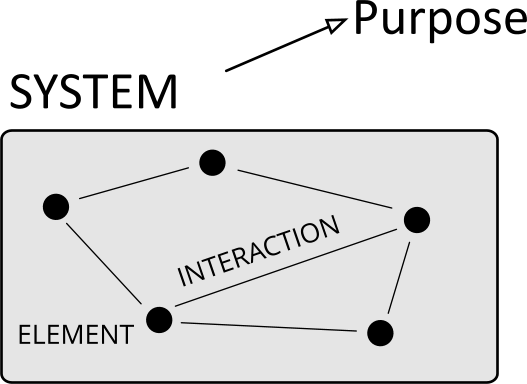
\includegraphics[width=.3\textwidth]{img/IMFmanual-img003.png}
  \caption{The system concept from ISO/IEC/IEEE
15288, illustrated as a group of elements interacting within a boundary to achieve a purpose.}
  \label{fig:Figure 3}
\end{figure}

As an example, the elements of a cooling system may be equipment such as pumps, pipes, chillers, etc. The purpose of the cooling system can be described as heat exchanging.

Below are observations  about purpose, elements, and interaction, followed by an observation about the system concept as a structuring principle.  These observations motivate  key ideas behind  IMF. 

\subsection{Purpose}
A system purpose can be described by stating an activity that the system is designed to bring about.
%In IMF an activity that describes purpose is called a primary classifier. 
Closely related to purpose is the concept of a system function, understood as 
%IMF follows IDO in understanding a system function as 
a capability of the system to realize its purpose. In IMF a system function is described indirectly
by describing the activity in which the function is realized, ie. by
stating  system purpose.

An engineered system will typically have medium at input and output, where 
medium is understood to be either material, energy, force, or signal carrying information.
Its purpose will  be described as an activity that transforms 
input media state to output media state. 

\subsection{System elements}
System elements can themselves be systems. In consequence, a system element of a system may be considered as a system with its own system
elements (illustrated in \autoref{fig:Figure 5}). This view of a system can be applied recursively, with system elements being
drilled down into sub-systems until a desired level of detail is achieved. The process of drilling down a system
element of one system to a system with its own system elements is called a \emph{system breakdown}. 

\begin{figure}[htb]
  \centering
  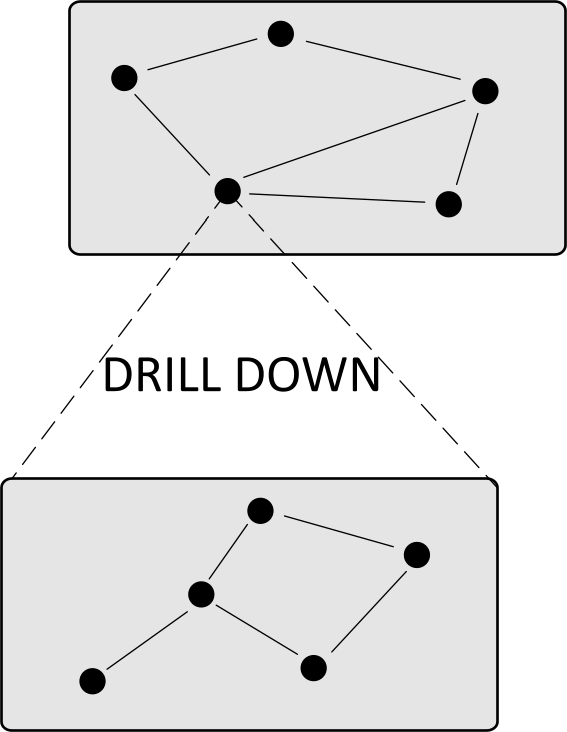
\includegraphics[width=.3\textwidth]{img/IMFmanual-img005.png}
  \caption{Illustration of a system breakdown}
  \label{fig:Figure 5}
\end{figure}

For example, a cooling system for an oil and gas facility might consist of a circulation system for the cooling medium and a heat
exchanger with seawater supply. The circulation system can be drilled down into a set of circulation pumps,
distribution headers and cooling medium expansion tank. All these system elements in the circulation system can be
further drilled down in new system breakdowns (e.g., cooling medium expansion tank system consists of valves and
instruments). 

% \textcolor{blue}{
The desired granularity of breakdown might vary between the different parties involved in the engineering of a facility asset. 
For instance, an engineering contractor may take the pump as an equipment that serves as a system element, while the pump supplier needs to view the pump as a system and perform a further system breakdown. Note that since the system elements of a system comprise a group, a breakdown is also a way of grouping.

\subsection{System interaction}
A system \textit{topology} describes how system elements are interconnected and hence how they interact. In IMF it is assumed
that system elements interact through media. 

Different disciplines will typically have focus on different media. Process engineers may, for example, be interested in how
the liquid and gas flow between system elements. The topology within a process system may hence be focused on these
types of media. An electrical engineer will be interested in how the electricity flows between the system elements
and design the topology of an electrical system accordingly.
The functions provided by a complex system   typically arise from interaction across different disciplines.
% At a higher level of abstraction, a system may group elements from different disciplines, 
Such systems can
be broken down into sub-systems where the system elements interact through only one single media type. This situation is illustrated in
\autoref{fig:Figure 6}. 
% Note that the principles for interaction across systems are the same as the principles of interaction within a system boundary. Baifan: "the same as the principles" is ambiguous, here principles can also be understood as phyiscal laws of different disciplines, which are certainly different across the sub-systems.

\begin{figure}[htb]
  \centering
  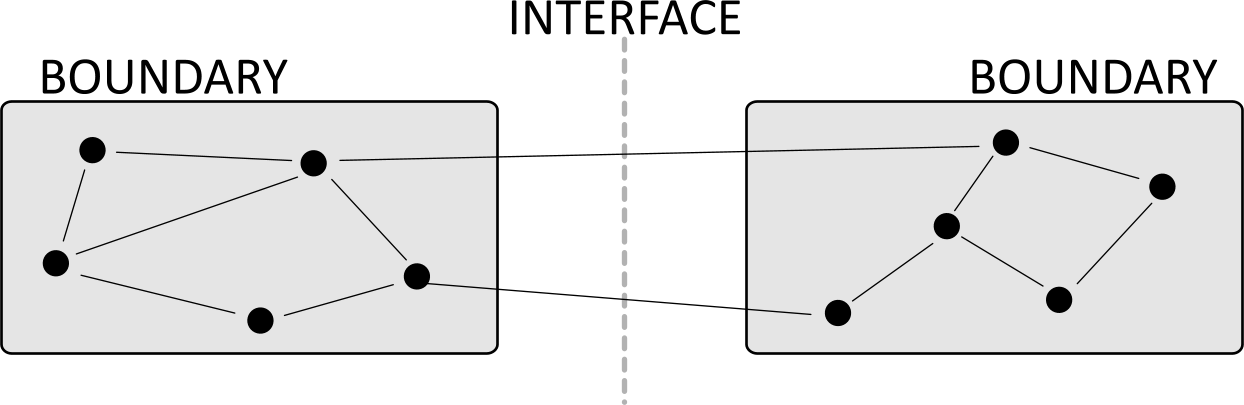
\includegraphics[width=.7\textwidth]{img/IMFmanual-img006.png}
  \caption{Illustration of the interaction of system elements
    inside and outside of system boundaries.}
  \label{fig:Figure 6}
\end{figure}

In the cooling system example, the pump and the heat exchanger interact by means of the cooling medium that the pump
pumps to the heat exchanger. The circulation pump is connected to an electric supply; thus, the cooling system
interacts with the electrical supply system of the facility.
 
The interface between two systems specifies how the systems interact. 
In IMF an interface is broken down to a set of connectors. Each
connector details the flow of a medium between two elements, e.g., how much cooling medium the pump shall supply 
to the heat exchanger. When IMF is used to describe functional requirements to a system,  
information on a connector 
can be understood as a description of a contract between the systems elements. 
  System elements of a system connect to elements outside the system boundary in the same way as they connect to system elements within the system boundary.
  
\subsection{The system concept as a structuring principle}
\label{sec:The_system_concept_as_structuring_principle}
An information model that describes an engineered system must describe its purpose, identify the elements that lie within the system boundary, classify these elements, and describe how these elements interact with each other and with elements outside the system boundary for the system to achieve its purpose. 

The system concept can be used as a structuring principle 
for developing  information models of engineered systems. Repeated use of the principles of system breakdown and interaction, as a recursive scheme, gives rise to  patterns
recurring at progressively smaller scales both vertically (system breakdown) and horizontally (system interactions) as is illustrated in \autoref{fig:Figure 7}.

\begin{figure}[htb]
  \centering
  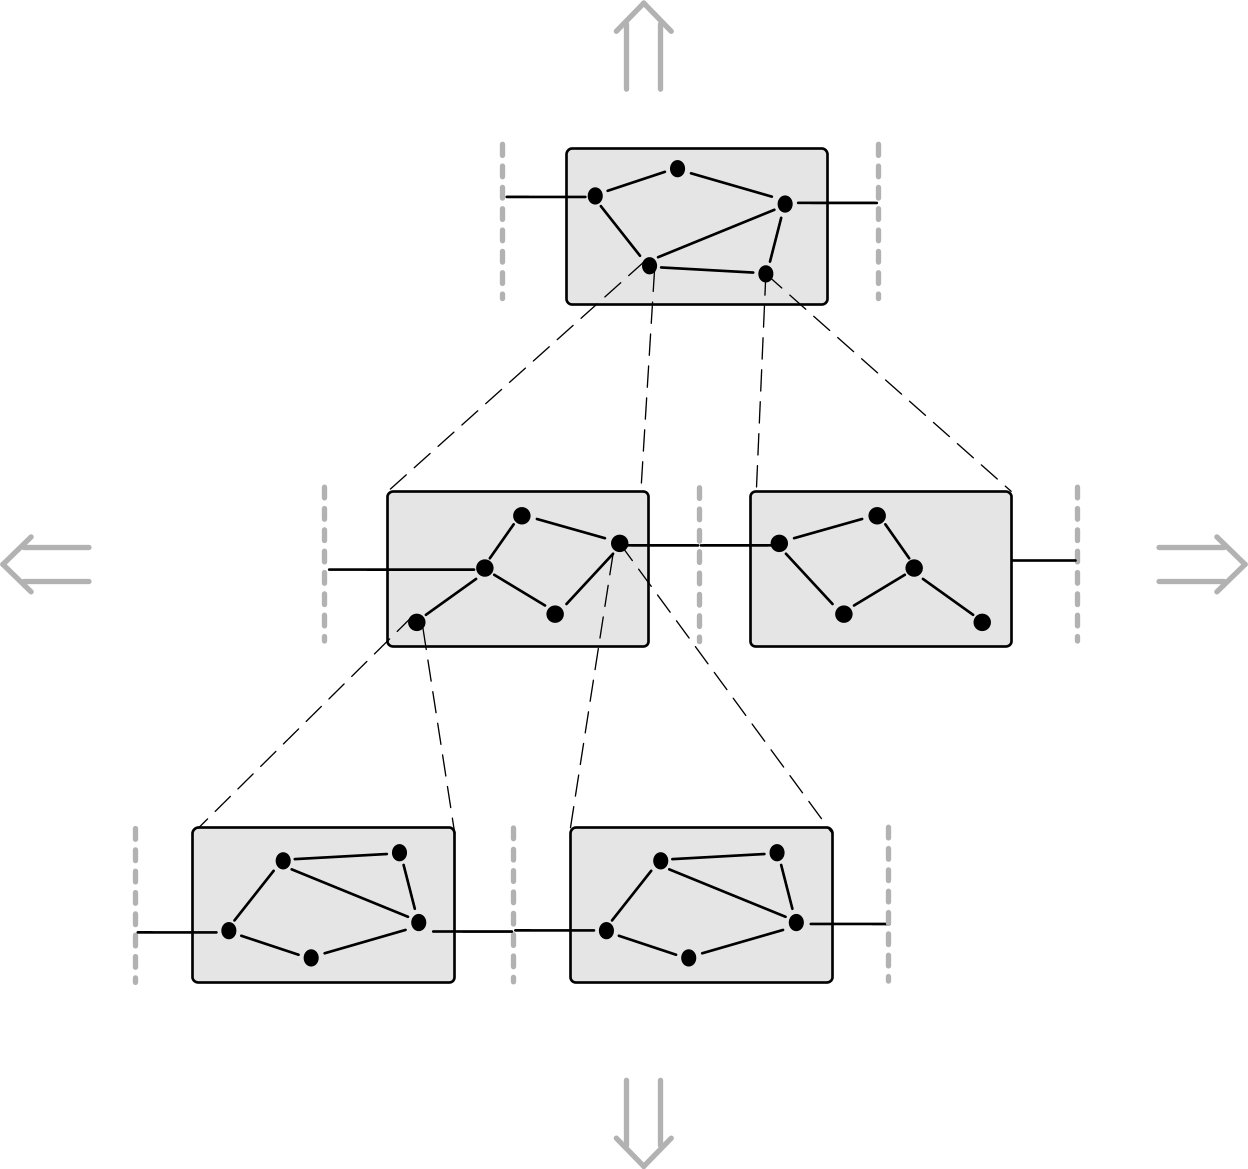
\includegraphics[width=.7\textwidth]{img/IMFmanual-img007.png}
  \caption{Illustration of system breakdown and topology.}
  \label{fig:Figure 7}
\end{figure}



Note that:
\begin{itemize}
    \item  A system may be broken down in more than one way, and hence give rise to different groups of system elements;
    \item A system  may be a system element of more than one system, and hence be part of more than one breakdown, 
    \item A system may be connected to other systems through more than one topology.
\end{itemize}
This ambiguity complicates both the design of information models, and access to technical information through them, since a user must manage different breakdowns and topologies without confusion.

Example: Consider a cooling system with, among other things, a pump connected to a heat exchanger.  The cooling system can be drilled down in several ways:
\begin{itemize}
    \item Functionally, the pump and the heat exchanger  are both contributing to a  function the cooling system and are hence contained in a function breakdown. 
    \item The pump can be delivered on a skid as part of a pumping package and hence be part of a bill of material breakdown of the engineering implementation. The heat exchanger may be delivered in a different package. 
    \item The pump can be located in an explosive area and is hence contained in an area breakdown. 
\end{itemize}
There are several topologies in play in the cooling system, for instance:  
\begin{itemize}
    \item The cooling medium of a pump  can be  represented by a connector with information about the cooling medium.
    \item The terminal of the pump is functionally connected to the terminal of
the heat exchanger. 
\item The terminal of the pump is  physically connected to the pipes that transport the cooling medium
through flanges that connect by means of mechanical force. 
\end{itemize}

%\comment{Example of different interests: different breakdown at different places in lifecycle. Example of different modes: actual, intended, simulated}

The IMF approach explained below is to use aspects to separate  different ways of  breaking down and connecting so that breakdown and connectivity  are not allowed to cross aspect. Each
element of a given aspect will then be part of a unique breakdown
hierarchy. This gives the intuitive operations of zooming in and
zooming out a precise meaning that can be implemented by traversing a
breakdown hierarchy upwards or downwards.
Also, a terminal of an aspect will be connected to a unique connector. 
Aspects can thus be used to resolve the ambiguity inherent in the system concept.  

\section{Aspect}
\label{sec:fundamentals_aspect}

IMF is  a language that can be used to describe assets from different points of view.  It is thus assumed that information about an asset is comprised of information from a multitude of views.  An IMF model aims to preserve these views and put them in relationships, and thus build them into the structure of IMF information models. 

\subsection{Definition of aspect}
An aspect is defined figuratively as a point of view.  The first task in making an IMF model is to define the aspects that will be used in the model. The definition of an aspect has to answer three questions:
\begin{itemize}
    \item What is the  information domain of the view?  There are three predefined information domains: Activity, Implementation, Space. 
    \item What is the modelling interest? There two two predefined interests: Product Lifecycle  and Project Lifecycle. 
    \item What is the mode of existence of what is modelled? There are two predefined modalities: Intended and Actual. 
\end{itemize}

The three dimensions in the definition of aspects are complementary. They are also extensible in the sense that more terms can be added when more detailed aspects are needed. 

\subsubsection{Information domain}
Information domain refers to what is captured in a view.
An information domain can be thought of as a filter on information. 
IMF has three predefined information domains and allows users to introduce more:
\begin{itemize}
    \item \textit{Activity}: Information about, e.g., process, motion, change. System purpose is meant to be captured in  terms of the Activity information domain; 
    \item \textit{Implementation}: Information about physical objects or software. A system view of elements as physical objects or software can be described in terms of the Implementation information domain;
    \item \textit{Space}: Information about, e.g., geometry, geographical position, what is located within what. Information about the space that an asset occupies is meant to be captured in terms of the Space information domain.
\end{itemize}

\begin{figure}[htb]
  \centering
  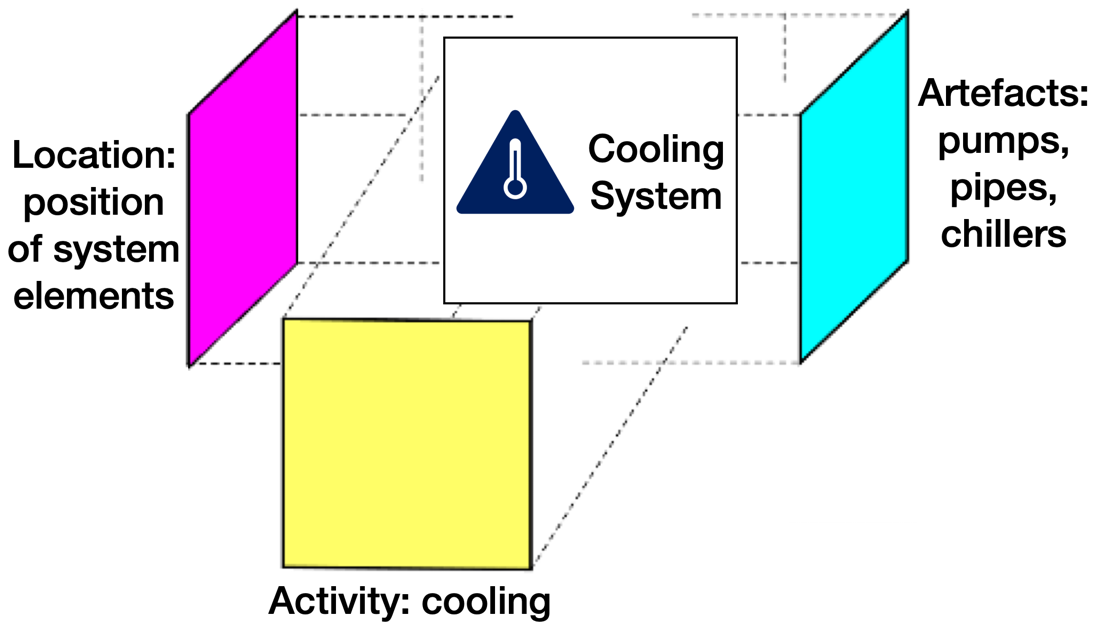
\includegraphics[width=.6\textwidth]{img/IMFmanual-img004.png}
  \caption{Different information domain views on the same system.}
  \label{fig:systemperspective}
\end{figure}



\autoref{fig:systemperspective} illustrates how the information domains can be applied to information about a cooling system as delivered from a supplier. 
In an  Activity information domain view, a cooling system is the cooling activity that realises the cooling function. 
In an  Implementation information domain view, a cooling system is comprised of physical system elements, such as pumps, pipes, and  chillers.
In a Space information domain view, a cooling system is the geometric extension of each of its physical system elements.

%function = capability to bring about an activity. An function is realised in an activity

Elements of, respectively, the Activity, Implementation, and Space information domains stand in different breakdown structures:
\begin{itemize}
    \item An Activity can be broken down into sub-activities;
    \item An Implementation can be broken down into sub-assemblies;
    \item A Space can be broken down into sub-spaces. 
\end{itemize}
Elements of the respective information domains are connected in different topologies: 
\begin{itemize}
    \item Two elements of the Activity information domain can be connected through a medium;
    \item Two elements of the Implementation information domain can be physically connected by being mounted together; 
    \item Two elements of the Space information domain can be connected by being adjacent or overlapping. 
\end{itemize}


\subsubsection{Interest}
The \textit{interest} is the modelling purpose; it points to the intended usage of the information, the users of the information and  their preferences and working habits.  An interest will in many cases be used to capture a specific segment of technical information. 

In this IMF  Manual there are two predefined terms for interests related to positions in the lifecycle of engineered assets.
\begin{itemize}
    \item Project lifecycle: This is used when the interest is in identifying   needs in project exection and in operation  and maintenance;
    \item Product lifecycle: This is used when the interest is from a supplier or manufacturer viewpoint.
    
\end{itemize}
 Users can add more fine-grained terms whenever needed. The value chain may include more steps that  users may need to distinguish between like, e.g., contractor and client in the project execution, or sub-suppliers in the product lifecycle. The project execution may introduce terms for milestones like, e.g., as-built and as-commissioned.  

% Each interest will be further elaborated in future versions of the IMF manual, and aligned to a system lifecycle ontology introduced in the future.

A fine-grained set of interest terms
%,  such as system design, detailed engineering, requirement engineering, manufacturing, procurement, commissioning, built, operation, maintenance, disposing, 
will provide users with  narrow contexts. This will, however, also give rise to many different aspects in the language, and a potential need for integrating information across aspects. 

%Since the interest contains the information of purpose, usage, and users, it also provides  principles of system modelling with breakdown and interaction, and hence how the system elements will be hierarchically grouped and broken down, and how the interactions shall be understood. 

\subsubsection{Modality}
The modality refers to the mode of existence of what is modelled. There are two predefined terms.
\begin{itemize}
    \item Intended: Information that expresses needs, specifications, or similar  engineering related information.    
    \item Actual: Information about physical assets.
\end{itemize}
Users may add other modalities. A Required modality may be useful in engineering.  In a digital twin context, a Simulated modality may be useful. 


\subsection{IMF aspects}
An IMF aspect is  defined  as as a triple: {\textless}\textit{Information domain}, \textit{Interest}, \textit{Modality} {\textgreater}.  

\autoref{tab:IMFaspectsIntended} lists the six combinations of predefined information domains and interests
for modality Intended. Here are some examples of what kind of information that can be captured in each of these aspects: 
\begin{itemize}
    \item Activity need: Functional requirements resulting from simulation. Breakdown of
    activities to a level of detail where a system function can be identified with capability to
    deliver the needed activity. Activity needs are typically activity breakdown hierarchies identified by the disciplines with interfaces to one another that bring details on various sorts of medium. 
    \item Area need: Definition of activity spaces and detailed positions and coordinates. The information will typically be organised in breakdown hierarchies with information about how they are interrelated, e.g., where they overlap or where they are adjacent. 
    \item Plant: Components and how they are physically assembled and connected. 
    \item Inherent function: The capability of a product  individual for bringing about an intended activity; the purpose of the product.  
    \item Product location: The space that product  individual occupies.
    \item Product type: The configured product template. 
\end{itemize}

\begin{table}
    \centering
    \caption{IMF aspects with modality Intended.}
    \label{tab:IMFaspectsIntended}
       %\resizebox{\textwidth}{!}{
    \begin{tabular}{llll}
     \toprule
        \textbf{Aspect short name}  & \textbf{Information domain} & \textbf{Interest} & \textbf{Modality}\\ \midrule
         Activity need&  Activity & Project Lifecycle & Intended\\
         Area need&  Space & Project Lifecycle & Intended \\
         Plant&  Implementation & Project Lifecycle & Intended\\
         Inherent function &  Activity & Product Lifecycle & Intended\\
         Product location&  Space & Product Lifecycle & Intended \\
         Product type &  Implementation & Product Lifecycle & Intended \\
     \bottomrule
    \end{tabular}
    %}
    
\end{table}

Example. In the lifecycle of an asset it may be important to distinguish between client needs and what is delivered by suppliers. IMF allows users to distinguish between  client and supplier interests and thus make information related to each of them be expressed in different aspects. Note that information about  client needs is not identical to product information from suppliers, even when this is information about the same asset and both client and supplier are using, e.g., the Activity information domain. 

\subsection{Reserved Aspects and ISO/IEC 81346}

The IMF manual uses reserved names for four aspects that have undefined interest, see  \autoref{tab:fouraspects}.
%the following four aspect definitions (\autoref{tab:fouraspects}):
%\begin{itemize}
%  \item        Function Aspect = {\textless}Activity, none, Intended{\textgreater}
%  \item        Product Aspect = {\textless}Implementation,  none, Intended{\textgreater}
%  \item        Location Aspect = {\textless}Space, none, Intended {\textgreater}
%  \item        Installed Aspect = {\textless}Implementation,  none, Actual {\textgreater}
%\end{itemize}
Colours are included in the table and are used in later figures in the IMF Manual to show the aspect. 



\begin{table}[tb]\centering\caption{Definition of  four aspects with no specific interest, and their
    prefixes and colours.}\label{tab:fouraspects}
    %\resizebox{\textwidth}{!}{
  \begin{tabular}{l lll c l}
    \toprule
\textbf{Aspect}  & \textbf{Information domain} & \textbf{Interest} & \textbf{Modality} &  \textbf{Prefix}  & \textbf{Colour} \\ \midrule
Function Aspect (F) &  Activity &none& Intended  &  =  &  yellow \\ 
Location Aspect (L)  & Space&none& Intended  & +  & magenta \\ 
Product Aspect (P) &  Implementation & none& Intended &  - &  cyan \\ 
Installed Aspect (I)  & Implementation&  none & Actual  & ::  &  dark blue\\
\bottomrule
  \end{tabular}
%}
\end{table}

\autoref{fig:Figure 8} illustrates these aspects applied to a pumping system.
\begin{itemize}
  \item The \textit{Function Aspect} (yellow) \ding{182} is used to specify the information about  activity that realises the function of the pumping system.
  \item The \textit{Product Aspect} (cyan) \ding{183} is used to specify the intended implementation of the pumping system.
  \item The \textit{Location Aspect} (magenta) \ding{184} is used to specify the %geometrical and positional information of the intended solution, e.g., the  
  size and shape of the specified pump. % and the requirements imposed by the location (ambient temperature etc. \baifan{I think the requirements posed by the location should go to function}).
  \item The \textit{Installed Aspect} (dark blue) \ding{185} is used to give information about the actual implementation, e.g., the serial number, run hours, and status of an actual pump installed in a plant.
\end{itemize}

\begin{figure}[htb]
  \centering
  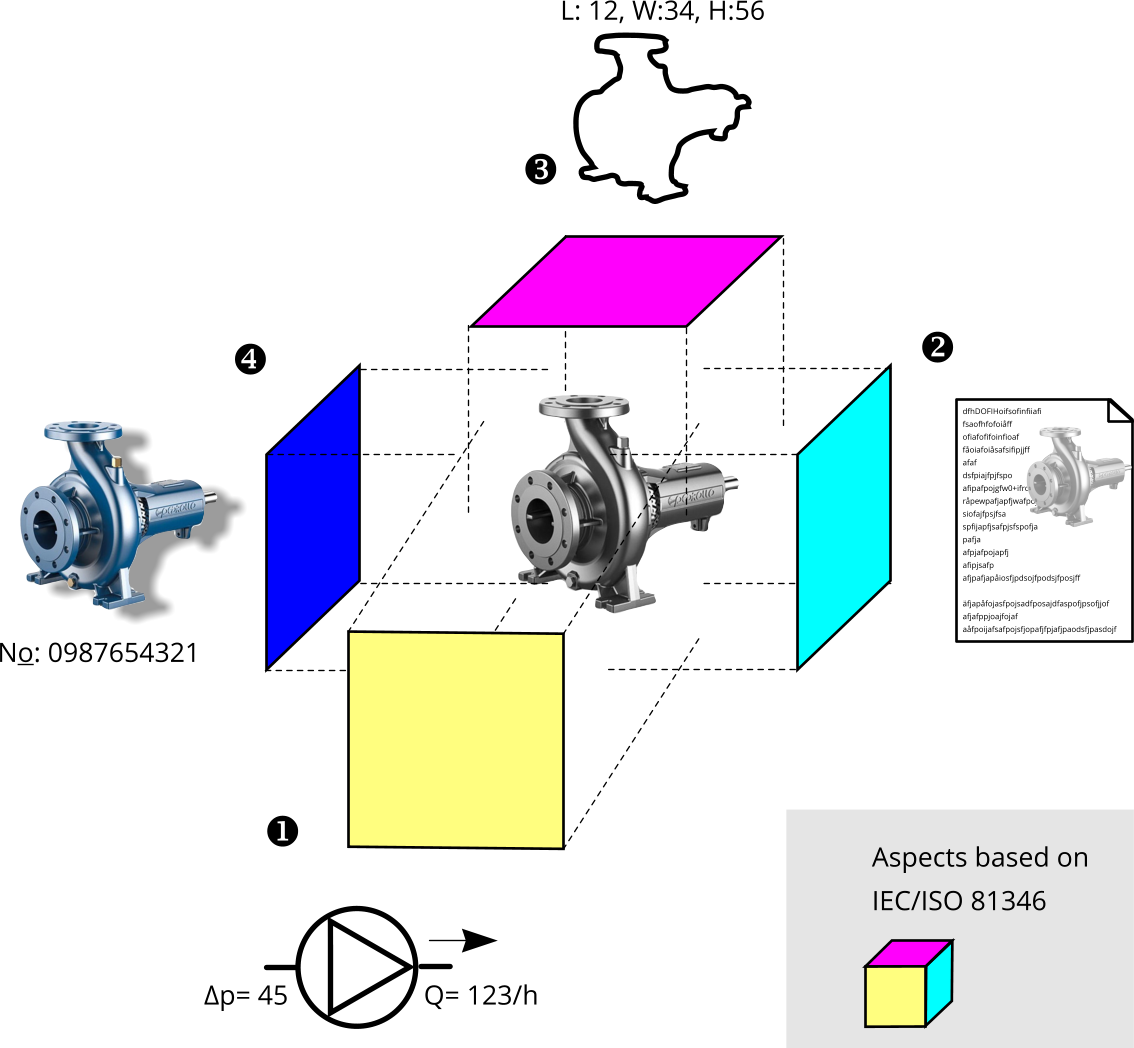
\includegraphics[width=.6\textwidth]{img/IMFmanual-img008.png}
  \caption[The concept of aspects.]{The four reserved aspects are illustrated: the Function Aspect (yellow), the Product Aspect (cyan), the Location Aspect (magenta), and Installed aspect (dark blue).}
  \label{fig:Figure 8}
\end{figure}


% Rewrite: 
% \textit{An Aspect is a particular way of viewing an object. There are at least four different Aspects, these are
%   listed in }\autoref{tab:fouraspects}\textit{. }


The Function, Product, and Location aspects of \autoref{tab:fouraspects} are identical to the core aspects of ISO/IEC 81346. These are the main differences between ISO/IEC 81346 and IMF on the treatment of aspects:
\begin{itemize}
    \item ISO/IEC 81346 does not have the IMF concept of interest. It does, however, allow introduction of new aspects. 
    \item ISO/IEC 81346 does not address individuals, and hence does not have the Installed aspect in \autoref{tab:fouraspects}. 
    \item ISO/IEC 81346 has a type aspect. IMF has a concept of type and a concept of classifier. The IMF concepts are not identical to the ISO/IEC 81346 type. 
\end{itemize}

\subsection{Describing systems using aspects}
\autoref{sec:The_system_concept_as_structuring_principle} identifies
limitations of the system concept as a structuring principle. The IMF approach to overcoming these limitations  is to define breakdown and topologies only within aspects, and allow users to flexibly flip between aspects. According to IMF principles,
\begin{itemize}
    \item An element of one aspect cannot be drilled down to an element of a different aspect.  A breakdown structure hence stays within an aspect;
    \item  An element in a breakdown structure can have at most one parent. 
    \item  An element of one aspect cannot be connected to an element of a different aspect. A topology hence stays within an aspect. 
\end{itemize}
A system will typically have different breakdowns and topologies in different aspects. But within one and the same aspect, there will be no ambiguity: 
\begin{itemize}
    \item An element can have at most one breakdown;
    \item An element is part of at most one breakdown;
    \item Two elements are connected through a topology in at most one way.
 \end{itemize} 
As a result, breakdown structures within aspects can be used to unambiguously zoom in when more detail is needed, and zoom out when a more comprehensive view is needed. This feature substantially facilitates navigation in technical information.

The definition of aspect provides users with flexibility to add new aspects  when this is needed for, e.g., an
element  in a breakdown structure to have just one parent. A user can in particular add an interest and form new aspects with this interest so that each element of this aspect has a unique breakdown.  

Note that the reserved aspects Function, Product, Location, and Installed will as a rule not be sufficient for meeting the  condition  that an element  in a breakdown structure can  have at most one parent.

In order to flip between aspects, IMF supports introduction of inter-aspect relations. One basic inter-aspect relation is the proxy relation. Two elements are said to be proxies if they 
are different views of the same thing, e.g., different views of the same system. 

\section{Information model}
\label{sec:InformationModel}
An  information model is an \textit{information artefact}, i.e. information that is constructed  in order to describe something. 
IMF models are  information models about assets that consist of \textit{elements} and \textit{descriptors} put into relationships by means of \textit{references}, \textit{relations}, and \textit{instantiations} of \textit{types}.

Both  elements and  relationships  result from applying  structuring principles that help organising engineering knowledge and technical information. In this process  identification of  elements, types, and descriptors is closely intertwined with identification of relationships. 

The full IMF language is presented in \autoref{ch:IMF visual language}. The aim of this section is to clarify principles that underlie some of the language constructs in IMF. 

\subsection{Element}
\label{sec:Element}
The IMF language contains three types of element: Block, Connector, Terminal.   

%\comment{Graphical symbols: FIGURE}

The elements are abstract forms that are useful for expressing simplified and aggregated views of technical information. Typically these views are  constructed by engineers using elements representing  concepts such as groups, systems, and specifications, and relationships between them. 
%i.e., \textit{part of}, \textit{connected to}, \textit{specialization of}, \textit{fulfills}, or \textit{instance of}. 
\begin{itemize}
    \item A block is used to represent anything of interest such as a system or a complex assembly that can  be divided into parts. 
    \item A connector is used to represent information about how two blocks  connect. When two blocks connect, they connect through a connector. A connector can in particular contain information about medium. 
    \item A terminal is  used  to express information about state of medium at the boundary of a block. 
\end{itemize}

%Each element can have classifiers. One of the classifiers is called  primary classifier. It is mandatory that this is given a value; if there is more than one mandatory classifier, all of them must apply to the element of which they are primary classifiers. An element can also have auxiliary classifiers.  

Blocks and connectors are associated with the concept of a boundary, intuitively meaning that any elements is, or is not, contained a  boundary. More precisely:
\begin{itemize}
    \item A block has a boundary.  
    \item A connector has a boundary.  
\end{itemize}
%A key intuition is that a connector holds information about how blocks can connect such that two blocks connect through a connector. Information on a connector can typically be understood as a specification of a protocol or contract between two blocks that connect through that connector. In particular information about medium can be represented as information on connectors.  
The connector is an element that can be present in a model even if it is not  connected to a block. This is not the case for terminals:
\begin{itemize}
%    \item A terminal  holds information about the state of medium at the boundary of the block.
    \item A  terminal can only be placed  at the boundary of a block. A connector cannot have terminals at its boundary.
    \item A terminal does not have a boundary.
\end{itemize}


\subsection{Descriptor}
\label{sec:Descriptor}
A descriptor is a term defined in IMF that is meant to be shared across models and use cases. Using references (cf. \autoref{sec:References}), both elements and other descriptors can refer to descriptors. IMF contains two types of descriptors:
\begin{itemize}
    \item Aspect, with the associated descriptor types  InformationDomain, Interest, and Modality, cf. \autoref{sec:fundamentals_aspect};
    \item Attribute, including Attribute Group and Attribute Qualifier, cf. \autoref{sec:attributes}.
\end{itemize}


\subsection{Reference}
\label{sec:References}
A reference is a term that is used to relate elements and descriptors to descriptors or external resources. %Three reference terms are classifier, hasAspect, and hasAttribute. 

%\subsubsection{classifier} \label{sec:classifier}
A \textit{classifier} is a reference that only elements can have. Classifiers detail  what the element at hand expresses information about. A classifier refers to an external resource such as a class in a reference data library or in an industry standard. 

All IMF elements have a mandatory classifier called the primary classifier.  They can also have any number of auxiliary classifiers. 

%\comment{Block example: Pumping. IP protection? one attribute? }
%\comment{Terminal and connector example? }

%Details on classifiers and attributes can either be defined for the IMF elements or be defined in reference data that the IMF elements refer to. It is hence possible to specify a division of labour between the IMF model and reference data that is appropriate for the users as regards where classifier details are expressed. 

Relationships between classifiers, such as the subclass relationship, are not expressed in IMF, but can be expressed in a reference data library. We may think of  relationships between classifiers as objective expressions about what something is, e.g., that a pump is a rotating equipment. If the reference data library is  structured in, e.g., subclass hierarchies, this structure can exploited  for verification and quality checking of  IMF models. 

%\comment{Example: Pumping and Mixer}

%\subsubsection{hasAspect}
An element can have a reference to an Aspect descriptor and thereby specify that it is of the given aspect. If an element is of an aspect, then this aspect is unique. 

Aspect details the view on technical information that is expressed through information about the element. Aspects regulate how users can build relationships between elements, e.g., by breaking something down in parts. We may think of such relationships as expressing subjective views,  shared by actors with the same interest, on the structure of technical information. 

%\subsubsection{hasAttribute}
An element may optionally have references to attribute descriptors.

\subsection{Relation}
\label{sec:Relations}
IMF is designed to facilitate operations on asset information in the engineering workflow through relations between elements. Three such operations are:
\begin{itemize}
     \item Flipping between abstraction layers,   facilitated by \textit{part of} relationships;
     \item Tracing medium flow, facilitated by  \textit{connected to}  relationships;
     \item Tracing requirement-solution threads, facilitated by \textit{fulfills}  relationships.
 \end{itemize}

%\begin{itemize}
%    \item Hierarchical relations 
%    \item Associative relations
%    \item IntraAspectRelations (Aspect-restricted relations)
%    \item Inter-aspect Relations
%    \item Constraining relations through aspects
%\end{itemize}
 
%\subsubsection{Relational structures in asset information}
%Organising asset information is an important task in the engineering workflow. In particular for systems engineering there is a need for organising  different sources of information in order to access the information needed for an engineering task at hand, extract relevant parts of it, and consolidate. In such workflows  engineers perform repeated operations on  various pieces of asset information, such as:

%IMF is designed to facilitate these four operations on asset information by providing language and methods for representing asset information in information models and building a relational structure into the models that directly reflects the four operations above. The structure is build using  relationships that can be expressed in the IMF language: 

\subsubsection{The \ow{partOf} relation}
%and \ow{containedIn} relationships}
Different abstractions are typically organised in breakdown structures. Something identified as an element in one source of technical information can be part of a group or system in another. The partOf %and containedIn 
relationship relates elements in breakdown structures. 

The concept of a boundary can provide intuitions on how  %containment  and 
division into parts is understood in IMF: 
\begin{itemize}
  \item A block can contain blocks, connectors, and terminals inside its boundary.
  \item A block can contain terminals at its boundary.
  \item A connector can contain blocks, connectors, and terminals inside its boundary, but a connector cannot contain a terminal at its boundary.
  \item A terminal can contain other terminals, but a terminal cannot contain blocks or connectors. 
\end{itemize}
%\comment{State rules for containment/partOf terminals here?}
%An element \textit{a} is \ow{containedIn} an element \textit{b} if \textit{b} contains \textit{a}. 
A breakdown hierarchy is represented as a sequence of \ow{partOf} relationships such that if A is \ow{partOf} B, then A is contained in B. 
%\textit{a} \textit{b}

%The \ow{partOf} relation is a sub-relation of \textit{containedIn}, which means that if an element A is \textit{partOf} an element B, then A is \textit{containedIn}  B.
%The \ow{containedIn} relation is transitive: If A is \textit{containedIn} B and B  is \textit{containedIn} C, then A is \textit{containedIn} C. The \textit{partOf} relation is not transitive, but related to \textit{containedIn} in the following way: 
%\begin{itemize}
%    \item If \textit{a} is \ow{containedIn} \textit{b}, then there is a chain of invervening elements between \textit{a} and \textit{b} such that the elements in the chain stand in pairwise \textit{partOf} relationships.
%    \item If there is a chain of invervening elements between \textit{a} and \textit{b} such that the elements in the chain stand in pairwise \textit{partOf} relationships, then \textit{a} is \ow{containedIn} \textit{b}.
%\end{itemize}

%\comment{Figure with boxes inside boxes and the same boxes in tree-shape with partOf.} 

In IMF an element can have at most one \ow{partOf} parent. Ie., if A is \ow{partOf} B, and C is different from B, then A cannot also be  \ow{partOf} C.  The \ow{partOf} relation is so-called \ow{functional}. 

The \ow{partOf} relation cannot relate elements of different aspects. 

%By applying the containment pattern in a recursive way we can construct a breakdown hierarchy that intuitively organises abstractions at different level of detail. For each step  where the  containment pattern is applied, an element is divided into parts. This gives rise to a partOf relation. Formally, the containment relation is defined through the partOf relation: 

\subsubsection{The \ow{connectedTo} relation}
Engineering artefacts such as products, systems, models, or elements in breakdown hierarchies  will in general be connected in different ways using  media types such as material, energy, force, or information. Traces of the flow of a medium type are typically depicted in topology diagrams.

In IMF a block and a connector can be connected via a terminal.  Information about media on connectors gives rise to topologies understood as a chain of connectors that represents the flow of medium.

The \ow{connectedTo} relation cannot relate elements of different aspects.
%\subsubsection{The \ow{specialization of} relationship}

\subsubsection{The \ow{fulfills} relation}
IMF uses the \ow{fulfills} relation to state a requirement-solution relationship between two elements. It can relate elements of different aspects. 

Engineering consists of a series of decisions whereby a solution space is successively constrained. An element of a design specification can be a solution to some requirements and itself pose new requirements for solutions as part of the gradual evolution of the engineering of an asset. Information in specifications such as data sheets can in many cases be traced back to elements of requirement specifications referring, e.g., to industry standards.

%\begin{itemize}
%    \item Element B specialises element A
%    \item Element B fulfils element A
%\end{itemize}
%Specialisation is expressed within an aspect; fulfilment can also be defined between elements of different aspects. 

Important to note is that the same set of information can be requirement for some group of information user, and at the same time intended solution for another group of information users. For example, in procurement
\begin{itemize}
    \item Client or contractor may provide a datasheet about some product to specify the required product requirement. The client datasheet will select information from the aspect Activity need, Area need, and Plant. 
    \item Supplier provides a datasheet about an offered solution based on some product catalogue of sub-supplier. The supplier datasheet will select information from the  Inherent function, Product location, and Product type aspects.
\end{itemize}

%Then the supplier B provides the datasheet about some product type based on some product catalogue that the supplier B can deliver (intended solution). The datasheet with the modality requirement will be verified against the datasheet provided with the modality intended solution. The later one then can serve as the requirement for the internal units of the supplier B, or the supplier C of the supplier B. 
% Another example: in commissioning (an interest), the information of artefacts installed in a factory is a description of the actual system (a description). This information will be verified against the information of the client that specifies the requirements for the system (a specification).
% Note. Information is used in integrity checking of IMF models. 

The evolving of information typically follows that in \autoref{fig:modalityevolve}: for the initial requirement an intended solution is proposed; then both of them are evolved to the revised requirement in the next stage, for which again an intended solution is proposed. This revision repeats until at the end an actual solution is installed. 
These relationships can be expressed in an IMF model using \ow{fulfills} relationships.

\begin{figure}[htb]
  \centering
  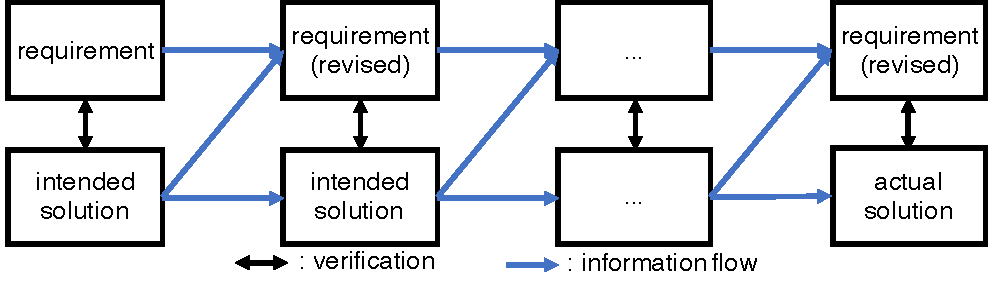
\includegraphics[width=.8\textwidth]{img/modalityevolve.pdf}
  \caption{The three modalities and a typical evolving flow}
  \label{fig:modalityevolve}
\end{figure}

%\subsection{instanceOf} \label{sec:instanceOf}
\subsection{Type and type instantiation}
\label{sec:Type}

 %\ow{instanceOf}


In all lifecycle phases engineers reuse patterns. In standardised design such patterns are called, e.g., design codes, typicals, or best practice. In commercial practice they may be called, e.g., modules, packages, or product types. 
These patterns are information structures that partially detail engineering solutions.
They can be found in libraries, standards, or other industry shared resources. 

An \emph{IMF type} is a predefined template for an information structure. It will typically contain elements with classifiers and attribute information, with or without values, potentially with a range of admissible values that an attribute may take. It will typically also contain information about connectors, and, in complex cases,  details about a breakdown into additional elements and a topology over those elements. 

Types in IMF are meant to reside in a library from which they can be accessed, instantiated, and reused. 
%Configuration. In the simplest case attribute values are inserted. In addition new attributed may be added. In complex cases more structure is added. 
%Instantiation: The configured type, with associated identifiers, is inserted into an IMF model. 
See Figure \ref{fig:Figure 38} for an illustration of how these ideas can be implemented and applied. 

In the current version of the manual, only elementary types are addressed, with the exception of the experimental text in Section \ref{sec: Employing Re-usable Design Patterns} and in Section   \ref{sec: What is an IMF Complex Type}. 

An element in an IMF model can be traced to types of which it is an instance. An element can in general be an instance of several types, and a type can instantiate several elements and relationships between them. 


\section{IMF concept and languages}
\label{sec:IMFconceptAndLanguages}

IMF allows users to construct information models using only three
element types. A restricted set of relations allows the user to
construct clearly defined breakdown hierarchies, topologies that
represent flow of medium, and requirement-solution chains through the
information model. Models can be composed by combining reusable types. By adding classifiers to elements,
classification hierarchies provided by external reference data
libraries can be exploited.
%, in particular for linkage to requirement specifications.

The IMF concepts are provided in different syntactic forms to
different user groups and for different purposes:

\begin{itemize}
    \item A visual language
    \item A formal RDF specification language
    \item An exchange protocol using AAS
    \item A formal semantics in formal logic
\end{itemize}

The focus of this document is the visual syntax.
%(RDF: resources that are referenced AAS, FOL: Not in this document note on graph and model. RDF Appendix?)

\textit{Visual language}. The purpose of the visual language is to provide an easy to use
language to the discipline experts to facilitate creation of
information models, navigation in such models, and formulation of
interesting views of a model.

The visual language is meant to be used in applications supporting
creation and manipulation of a simple set of graphical elements and
relationships for building graphs using a restrictive set of templates.
The resulting graphs are meant to be composed of recognizable links
between the elements that should be intuitively simple to navigate
through. When a specific view is of interest, the user should be
able to select elements and relationships of that view.
 
\textit{RDF representation.} The RDF representation captures the
meaning of an IMF model in a more precise way than the visual
language.  RDF is a W3C recommendation (ie. a standard for the
semantic web) for specifying graphs.  It enables the representation of
complex constraints that are useful for developers of applications for
the visual language; such constraints can help users avoid creating
patterns in the model that go against the intended meaning.

An expert in RDF can also write a graph pattern and, using the W3C
recommended query language SPARQL, pose this as a query to an RDF
graph; the query will then return patterns in the graph that match the
pattern of the query.  If the discipline expert specifies an
interesting view, the RDF expert can hence implement this view by
writing the corresponding query, execute this over the model, and visualize the query result to the user as a view of the information model. 

\textit{Exchange protocol}.
Information about assets is
fragmented; it is created in and exchanged between silos arising
between disciplines and along the value chain. When IMF models are
developed in silos, there is need for serialisations of the
models that can be effectively exchanged.

RDF is a serialisation format for the semantic web that can be used as
exchange protocol when it is supported.  Otherwise it is practical to
use protocols that the industry has already implemented.  This can be
supported in IMF by specifying a translation from the RDF
representation to the serialisation format at hand that preserves
model structures, i.e. a structure preserving translation.

The Asset Administration Shell is an industry implemented protocol for
exchange of information between supplier and client as part of the
Industry 4.0 program. The IMF project aims to support exchange of
model information using AAS by providing a profile to AAS. This is not
included in this version of the IMF manual.

\textit{Formal semantics}.
 By using formal logic, including
first-order logic, the meaning of IMF models can be expressed as rules
and constraints even more concisely than in the RDF
representation. The formal semantics is also referred to as the
interpretation of IMF.

Application developers can use the formal semantics to build logic
into applications.  Since formal semantics supports automated
reasoning, the formal semantics can also be exploited for powerful
integrity checking and formal verification.

In particular the formal semantics can provide a bridge to the
Industrial Data Ontology (IDO), which is particularly designed to
exploit the automated reasoning capabilities of the OWL, the web
ontology language recommended by W3C.  When elements of an IMF model
are classified using resources in a reference data library that
conforms to IDO, off the shelf automated reasoning tools can already
today provide very efficient and advanced integrity checking. IMF is
designed to enable such use of IDO and associated automated reasoning
services.

%OLD TEXT: If the reference data library is an ontology structured according to IDO, the IMF model can even exploit automated reasoning services over the reference data ontology. This can in particular be useful for checking that an element satisfies a requirement specification in cases where the requirement is triggered by membership in a class. Automated reasoning can in such cases be used to check if  an IMF element has a classifier that is a subclass of a class that triggers a given requirement, and hence check whether or not that requirement has been met. 
\end{document}
